\newpage
\section{Реализация драйвера}
\subsection{Обнаружение и включение устройства}

Перед началом работы, необходимо провести поиск и идентификацию устройства. В ядре Linux имеется достаточно богатый набор API для обнаружения устройств, использующих шину PCI (Plug \& Play). Функция pci\_find\_device (Листинг 1, строка 20) ищет устройство в списке устройств с заданной сигнатурой или принадлежащие к определённому классу. Если ничего не найдено, возвращается значение NULL.

\lstinputlisting[language=C++, caption={Обнаружение и включение устройства (res/r8169-alpha.c)}]
{res/r8169-alpha.c}

Каждый производитель имеет уникальный, назначенный только ему идентификатор ID и назначает уникальный идентификатор ID каждому конкретному виду устройств. Макросы REALTEK\_VENDER\_ID и REALTEK\_DEVICE\_ID (Листинг 1, строки 16 и 17) определяют эти идентификаторы ID. Найти эти значения можно в "PCI Configuration Space Table" в спецификациях RealTek8169\cite{Realtech}.

После того, как устройство обнаружено, то, прежде чем как-то с ним взаимодействовать, его нужно включить. 

Функция probe\_for\_realtek8169 (Листинг 1, строка 43) выполняет следующие задачи:

\begin{itemize}
\item Проверяет, что мы работаем на PCI-совместимой системе (pci\_present вернет NULL, если система не поддерживает PCI).
\item Пытается найти устройство RealTek 8169 так, как это показано в таблице 1.
\item Включает устройство (с помощью функции pci\_enable\_device), если его найдет.
\end{itemize}

\subsection{Инициализация устройства}

На прошлом шаге был разработан драйвер, который позволяет обнаружить и включить сетевое устройство. На данном шаге будет представлен драйвер, который будет способен инициализировать устройство.

Ранее была рассмотрена структура net\_device, содержащее поле priv. Объявим структуру, в которой будут храниться приватные данные устройства (листинг 2), а указатель на эту структуру должен храниться в поле priv.

\lstinputlisting[language=C++, firstnumber=40, firstline=40, lastline=45, caption={Структура rtl8169\_private (res/r8169-betta.c)}]
{res/r8169-betta.c}

В остальной части функции init\_module теперь можно определить указатель net\_device и инициализировать его (листинг 3).

\lstinputlisting[language=C++, firstnumber=47, firstline=47, lastline=152, caption={Инициализация net\_device (res/r8169-betta.c)}]
{res/r8169-betta.c}

Функция probe\_for\_realtek8169 (листинг 3, строка 82) была рассмотрена на предыдущем шаге. Функция rtl8169\_init (листинг 3, строка 50) распределяет память для локального указателя dev (листинг 3, строка 60), который должен использовать как net\_device. Кроме того, эта функция заполняет компоненту pci\_dev структуры rtl8169\_private (листинг 3, строка 67) для обнаруженного устройства.

Далее необходимо получить поле base\_addr для net\_device. Оно указывает на начало памяти регистров устройства, которые потребуются для реализации ввода-вывода с отображением в память. Чтобы получить базовый адрес для ввода-вывода с отображением в память, используем PCI API такие как pci\_resource\_start (листинг 3, строка 95), pci\_resource\_end (листинг 3, строка 96), pci\_resource\_len (листинг 3, строка 97), pci\_resource\_flags (листинг 3, строка 98). Эти API позволяют читать конфигурационное пространство PCI, не зная о деталях его реализации. Второй аргумент в этих API -- номер BAR. Согласно спецификации RealTek8169, первый BAR (нумеруемый как 0) -- I/OAR, тогда как второй BAR (нумеруемый как 1) -- MEMAR. Поскольку в этом драйвере используется ввод-вывод с отображением в память, то в качестве второго аргумента передаем 1.

Прежде, чем получить доступ к адресам, возвращаемыми указанными выше API, нужно должны сделать две вещи:
\begin{enumerate}
\item Зарезервировать в драйвере указанные выше ресурсы (пространство памяти); это делается с помощью вызова функции pci\_request\_regions (листинг 3, строка 108).
\item Отобразить адреса ввода-вывода (описанные выше) так, чтобы они использовались при вводе-выводе с отображением в память.
\end{enumerate}
Адрес ioaddr назначается компоненте base\_addr в структуре net\_device (листинг 3, строка 124), и это то место, откуда можно начинать читать регистры устройства или писать в них.

В оставшейся части кода из листинга 3, выполняется обычная инициализация структуры net\_device. Стоит отметить, что производится чтение аппаратного адреса из устройства и запись его в dev\_addr. Если изучить описания регистров в спецификации RealTek8169, то можно видеть, что первые 6 байтов являются аппаратным адресом устройства. Также нужно иметь проинициализированные компоненты указателя на функцию, но без определения какой-либо соответствующую функцию.

Теперь для компиляции модуля без ошибок, добавим пару заглушек (листинг 4).

\lstinputlisting[language=C++, firstnumber=154, firstline=154, lastline=176, caption={Функции-заглушки (res/r8169-betta.c)}]
{res/r8169-betta.c}

В init\_module пропущена обработка ошибок. В самом простом случае, она может выглядит так, как показано в листинге 5.

\lstinputlisting[language=C++, firstnumber=178, firstline=178, lastline=190, caption={Обработка ошибок (res/r8169-betta.c)}]
{res/r8169-betta.c}

На данный момент драйвер может включать устройство и отображать его в пространство пользователя. Можно откомпилировать его код и вставьте его в ядро (предполагается, что исходный код ядра - /usr/src/linux-2.4.22). Погрузка модуля в ядро (insmod) потребует прав суперпользователя.

\begin{Verbatim}[frame=single]
$ gcc -c rtl8169.c -D__KERNEL__ -DMODULE -I /usr/src/linux-2.4.22/include
$ sudo insmod rtl8169.o
\end{Verbatim}

\newpage
\subsection{Реализация функций приёма и передачи}

На предыдущем шаге была показана инициализация устройства, но функции приёма и передачи заменены заглушками. Теперь рассмотрим как осуществлять приём и передачу сетевого трафика.

В RealTek8169 имеется 4 дескриптора передачи, каждый дескриптор имеет фиксированное смещение адреса ввода-вывода\cite{Realtech}. Четыре дескриптора используются циклически. Это означает, что для передачи четырех пакетов драйвер будет использовать в циклическом порядке дескриптор 0, дескриптор 1, дескриптор 2 и дескриптор 3. Для передачи следующего пакета драйвер снова будет использовать дескриптор 0 (при условии, что он свободен). В спецификациях RealTek8169 указывается, что регистры TSAD0, TSAD1, TSAD2 и TSAD3 имеют смещения 0x20, 0x24, 0x28, 0x2C, соответственно. В этих регистрах хранится "начальный адрес дескрипторов передачи ", т.е. в них хранится стартовый адрес (в памяти) пакетов, которые должны быть переданы. Позже устройство считает содержимое пакетов из этих адресов DMA, перепишет их в свой собственный стек FIFO, а затем выполнит передачу данных в сеть. Таким образом, драйвер должен выделять память прямого доступа (доступ DMA), где будут храниться пакеты, и записывает адрес этой памяти в регистры TSAD.

Приемная часть RTL8169 спроектирована как кольцевой буфер (линейная память, управление которой осуществляется как кольцевой памятью). Всякий раз, когда устройство принимает пакет, содержимое пакета запоминается в память кольцевого буфера и изменяется место, куда будет записываться содержимое следующего пакета (начальный адрес первого пакета + длина первого пакета). Устройство продолжает так запоминать пакеты до тех пор, пока не исчерпается линейная память. В этом случае устройство снова начинает запись с начального адреса линейной памяти, реализуя, таким образом, кольцевой буфер.

Добавим в структуру rtl8169\_private поля, в которых будут храниться данные, связанные с передачей пакетов (листинг 6).

\lstinputlisting[language=C++, firstnumber=93, firstline=93, lastline=110, caption={Инициализация net\_device (res/r8169.c)}]
{res/r8169.c}

Компонента tx\_flag (листинг 6, строка 99) должна содержать флаги передачи, уведомляющие устройство о некоторых параметрах, которые будут рассмотрены ниже. Поле cur\_tx (листинг 6, строка 100) должно хранить текущий дескриптор передачи, а dirty\_tx (листинг 6, строка 101) указывает на первый из дескрипторов передачи, для которых передача еще не завершена (это означает, что мы можем использовать эти занятые дескрипторы для следующей передачи пакетов до тех пор, пока предыдущий пакет не будет полностью передан). В массиве tx\_buf (листинг 6, строка 102) хранятся адреса четырех "дескрипторов передачи". Поле tx\_bufs (листинг 6, строка 103) используется для тех же самых целей. В tx\_buf и в tx\_bufs должен храниться именно виртуальный адрес, который может использоваться драйвером, но устройство не может использовать такие адреса. Устройству для доступа нужен физический адрес, который запоминается в поле tx\_bufs\_dma (листинг 6, строка 104).

Компонента stats (листинг 6, строка 106) должна хранить статистику с устройства (большая часть статистики, выдаваемой ifconfig, берется из этой структуры). Следующая компонента, rx\_ring (листинг 6, строка 107), является адресом памяти в ядре, где запоминаются принятые пакеты, а rx\_ring\_dma (листинг 6, строка 108) -- физический адрес этой памяти. Компонент cur\_rx (листинг 6, строка 109) используется для отслеживания места, куда будет записываться следующий пакет.

Ниже (листинг 7) приведен список смещений регистров, используемых в исходном коде (более подробную информацию об этих значениях можно получить из спецификаций RealTek8169). Кроме этого, там размер памяти, нужный для кольцевого буфера (листинг 7, строки 6-14), используемого для приёма сообщений.

\newpage

\lstinputlisting[language=C++, firstnumber=6, firstline=6, lastline=50, caption={Определения регистров (res/r8169.c)}]
{res/r8169.c}

Теперь рассмотрим реализацию функций, работающих с устройством для передачи данных (листинг 8). Ранее эти функции были представлены простыми заглушками.

\lstinputlisting[language=C++, firstnumber=232, firstline=232, lastline=350, caption={Определения регистров (res/r8169.c)}]
{res/r8169.c}

Функция rtl8169\_open (листинг 8, строка 232) начинается с запроса IRQ, что делается вызовом API request\_irq (листинг 8, строка 241). В этой функции регистрируется обработчик прерываний rtl8169\_interrupt. Эта функция будет вызываться ядром всякий раз, когда устройство генерирует прерывание. Теперь выделим память, куда будут записываться исходящие пакеты, прежде чем они будут переданы в сеть. Вызов API pci\_allocate\_consistant возвращает виртуальный адрес ядра (листинг 8, строка 248). Физический адрес возвращается в третьем аргументе, который потом будет использован драйвером. Таким образом выделяется память для всех четырех дескрипторов. Функция rtl8169\_init\_ring (листинг 8, строка 279) распределяет эту память для четырех дескрипторов.

Теперь рассмотрим функцию rtl8169\_hw\_start (листинг 8, строка 293), которая делает устройство готовым для передачи (и приёма) пакетов. Сначала перезагружаем устройство для того, чтобы оно было в предсказуемом и известном состоянии (листинг 8, строка 299). Это делается с помощью записи в регистр команд CR (Command Register) значения reset (листинг 8, строка 339), что описано в спецификациях. Дождёмся, пока записанное значение можно будет считать обратно, что означает, что устройство перезагружено. Следующая функция, barrier(), вызывается с тем, чтобы ядро выделило память, требуемую для ввода-выхода, без какой-либо оптимизации (листинг 8, строка 344). Поскольку устройство перезагружено, можно записать в регистр CR значения CmdTxEnb | CmdRxEnb, что означает, что устройство будет передавать и принимать пакеты (листинг 8, строка 302). Затем сконфигурируем регистр TCR (Transmission Configuration Register -- конфигурационный регистр передачи) (листинг 8, строка 305). Единственное, что мы установим в регистре TCR, это "Max DMA Burst Size per Tx DMA Burst" (максимальный размер буфера DMA для каждого сохраняемого в DMA пакета). Все остальные значения оставим установленными по умолчанию (подробности в спецификациях). Теперь запишем DMA адрес всех четырех дескрипторов в регистры TSAD (Transmission Start Address Descriptor – дескриптор начального адреса передачи) (листинг 8, строка 315). Остальные строки пока останутся без комментариев. Они потребуется для передачи.

Далее включаем прерывания, сделав для этого запись в регистр IMR (Interrupt Mask Register – регистр маски прерывания) (листинг 8, строка 328). Этот регистр позволит задать, какие прерывания будет генерировать устройство. Наконец, вызываем netif\_start\_queue (листинг 8, строка 330) с тем, чтобы сообщить ядру, что устройство готово. Осталось лишь реализовать функцию rtl8169\_interrupt. Устройство уже готово посылать пакеты, реализация этой функции представлена ниже (листинг 9).

\lstinputlisting[language=C++, firstnumber=352, firstline=352, lastline=381, caption={Функция отправки пакетов (res/r8169.c)}]
{res/r8169.c}

Функция rtl8169\_start\_xmit (листинг 9, строка 352) крайне проста: сначала она ищет имеющийся дескриптор передачи, а затем проверяет, чтобы размер пакета был, по меньшей мере, 60 байтов (поскольку размер пакетов Ethernet не может быть меньше 60 байтов)(листинг 9, строка 359). Как только это будет сделано, будет вызвана функция skb\_copy\_and\_csum\_dev (листинг 9, строка 363), которая скопирует содержимое пакетов в имеющуюся память DMA. Следующая функция writel (листинг 9, строка 371) информирует устройство о длине пакета. После этого пакеты передаются в сеть. Далее определяем имеющиеся в наличии следующие дескрипторы передачи и, если он будет равен дескриптору, для которого передача еще не завершена (листинг 9, строка 376), то остановим устройство; в противном случае просто выйдем из функции.

Теперь устройство готово отсылать пакеты. Для приёма пакетов, вернёмся к листингу 8. В строке 308 производится конфигурирование сетевой карты для приёма сообщений (подробности есть в спецификации\cite{Realtech}):
\begin{itemize}
\item Бит 1 -- Принимаются пакеты с проверкой физического адреса (адреса MAC).
\item Бит 2 -- Принимаются многоадресные пакеты (посылаемые на несколько адресов)
\item Бит 3 -- Принимаются широковещательные пакеты (посылаемые на все адреса)
\item Бит 7 -- WRAP. Когда установлен в 1, то RTL8169 будет перемещать оставшуюся часть пакетных данных в память, которая следует непосредственно за концом премного буфера.
\item Биты 8-10 -- Максимальный размер буфера DMA для каждого сохраняемого в DMA пакета. Значение 111 соответствует отсутствию ограничений.
\item Биты 11-12 -- Длина буфера приема. Устанавливаем это значение равным 10, что означает 32K+16 байтов. 
\end{itemize}

Кроме того, стоит отметить конфигурирование регистра RBSTART (листинг 8, строка 319). В этом регистре содержится стартовый адрес приемного буфера. Далее обнуляем регистр MPC (Missed Packet Counter – счетчик ошибочных пакетов) (листинг 8, строка 322) и конфигурируем устройство так, чтобы не генерировались ранние прерывания (листинг 8, строка 325).

Последний важный момент, который нужно обсудить -- обработчик прерываний устройства. Этот обработчик прерываний ответственен за прием пакетов, а также за обновление необходимой статистики. Ниже (листинг 10) приведен его исходный код.

\lstinputlisting[language=C++, firstnumber=383, firstline=383, lastline=500, caption={Обработчик прерываний (res/r8169.c)}]
{res/r8169.c}

Как видно из листинга 10, регистр ISR будет считан в переменную isr (листинг 10, строка 388). Любое дальнейшее демультиплексирование прерывания -- это работа обработчика прерываний. Если принять прерывания TxOK, TxErr или RxErr, то потребуется обновить статистику. Прием прерывания RxOK означает, что мы приняли кадр успешно и драйвер обработал его (листинг 10, строка 437). Мы будем читать из приемного буфера до тех пор, пока не прочитаем все данные (эту работу выполняет цикл while в строке 440). Сначала проверим, не вышло ли значение tp->cur\_rx за длину RX\_BUF\_LEN (листинг 10, строка 447). Если это так, мы выставляем значение wrap. Первые два байта указывают статус кадра, а следующие два байта указывают длину кадра (длина также включает первые 4 байта)\cite{Realtech}. Эти значения всегда в обратном порядке и их следует преобразовать. Затем для принятого пакета выделяем место для skb (листинг 10, строка 462), копируем содержимое кадров в skb (листинг 10, строка 468) и ставим skb в очередь для дальнейшей обработки(листинг 10, строка 471). Затем обновляем CAPR (Current Address of Packet Read -- текущий адрес чтения пакета) с тем, чтобы устройство RTL8169 знало о месте следующей операции записи. Обратите внимание, что этот обработчик прерываний уже зарегистрирован в функции rtl8169\_open.

Таким образом, заглушки заменены полноценными функциями драйвера (Рисунок 2).

\begin{figure}[h!]
\centering
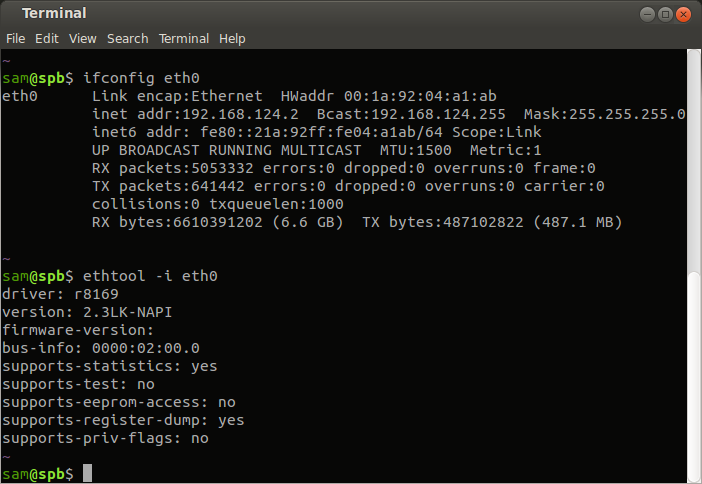
\includegraphics[scale=0.7]{res/pic02}
\caption{Работающий сетевой интерфейс}
\end{figure}

Полученный результат во многом совпадает с кодом, находящимся в ядре Linux, но проигрывает только по количеству проверок на ошибки. Кроме того, использует значительно меньше макросов для обеспечения наглядности.